\documentclass[10pt]{beamer} 
%\setbeamerfont{smaller}{size=\tiny } 
%\usepackage[latin1]{inputenc} 
\usepackage{verbatim}  
 \usepackage{graphicx} 
%\usepackage{multicolumn}

\usepackage{wrapfig}
%\usepackage{grahicx} 
\usetheme{Hannover} % Marburg, Berkeley, Berlin, Singapore 
\title{Optimizing paths in figure-8 task using reinforcement learning} 
\subtitle{\small Supervisor: Arnoud Visser} 
\author{Martijn van der Veen} 
\institute{University of Amsterdam} 

% \begin{block}{Block title} \begin{alertblock}{Alert-block title} \begin{exampleblock}{Example-block title}

% Color text for slide \colortxt{slide}{color}{text}
\newcommand{\colortxt}[3]{\only<#1>{\textcolor{#2}}{#3}}

\begin{document}

\begin{frame}
\begin{center}

%\includegraphics[height=2cm]{}%uva}

\end{center}
\titlepage
\end{frame}

% \begin{comment}
% % Uncover example
% Test\\
% \uncover<2-3>{Korte tekst tussendoor}
% \uncover<4->{Test2}
% ook leuk:
% \only<2>{}
% Dit toont iets op alleen 1 slide
% Je kan ook \pause gebruiken
% 
% MultiColumn output
% %\begin{columns}[l]
% %\column{1.5in}
% %\column{1.5in}
% %\end{columns}
% \end{comment}

\begin{frame}
\tableofcontents
\end{frame}

\section{Goal}
\begin{frame}
 \frametitle{Goal}
 Learn path of figure-8 challenge using reinforcement learning for aerial robot.
 \begin{figure}
  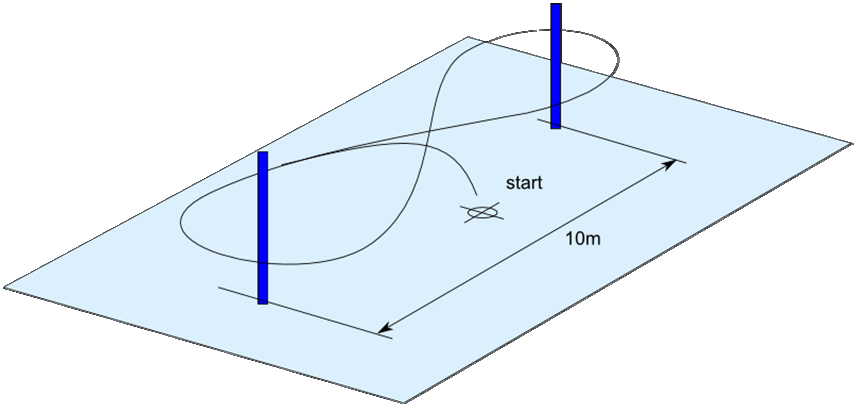
\includegraphics[width=0.8\textwidth]{img/imav2011_pylon}
 \end{figure}
\end{frame}

\begin{frame}
 \frametitle{Why?}
 \begin{itemize}
   \item Frequently used for testing (real) robots
   \item Task suitable for Reinforcement Learning
   \item Autonomous aerial systems are useful
   \begin{itemize}
     \item Locations humans / ground robots cannot reach
     \item Nice overview
     \item Price is dropping
   \end{itemize}
 \end{itemize}
\end{frame}

\section{Related Work}
\begin{frame}
 \frametitle{Related Work}
 \begin{itemize}
   \item Figure-8 mostly used for ground robots
   \item Often using SLAM
   \item Not much 'learning'
 \end{itemize}
\end{frame}

\section{Approach}
\begin{frame}
 \begin{itemize}
   \frametitle{Approach}
   \item Train in simulation, use in real life
   \begin{itemize}
     \item Unreal Tournament 2004 + USARSim
     \item AR.Drone ported to Unreal by Nick Dijkshoorn
   \end{itemize}
 \begin{figure}
  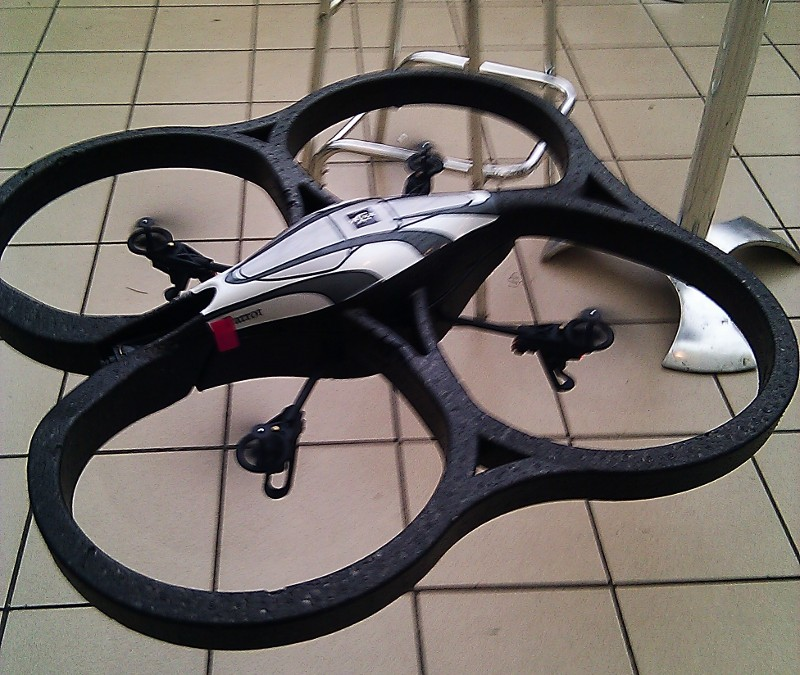
\includegraphics[width=0.3\textwidth]{img/ARDRONE}
 \end{figure}
 \begin{figure}
  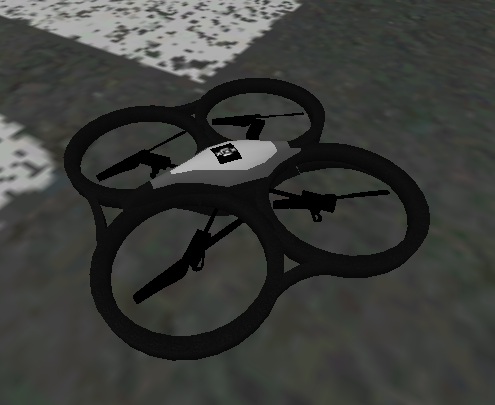
\includegraphics[width=0.3\textwidth]{img/ardrone_sim}
 \end{figure}
 \end{itemize}
\end{frame}

\begin{frame}
 \begin{itemize}
   \frametitle{Approach}
   \item Train in simulation, use in real life
   \begin{itemize}
     \item Unreal Tournament 2004 + USARSim
     \item AR.Drone ported to Unreal by Nick Dijkshoorn
   \end{itemize}
 \begin{figure}
  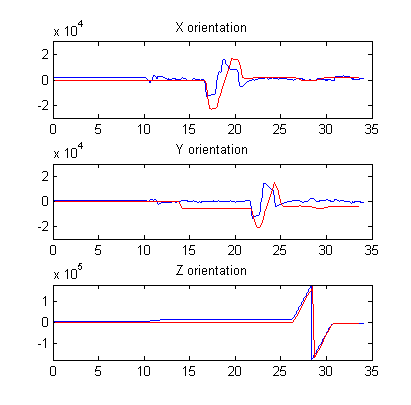
\includegraphics[width=0.7\textwidth]{img/ardrone_real_sim}
 \end{figure}
 \end{itemize}
\end{frame}

\begin{frame}
 \begin{itemize}
   \item Train in simulation, use in real life
   \begin{itemize}
     \item Unreal Tournament 2004 + USARSim
     \item AR.Drone ported to Unreal by Nick Dijkshoorn
     \item Switch between simulation and real life
   \end{itemize}
   \item Learn 'Force Field'
   \pause
   \item Set initial force field
   \pause
   \item Use different stages / force fields (crossed path)
   \pause
   \item Use reinforcement learning
 \end{itemize}
\end{frame}

\begin{frame}
  \begin{itemize}
   \item No states but forces
   \begin{figure}
    
\includegraphics[width=0.1\textwidth]{img/rl_force}
   \end{figure}
   \item Rewards: +10 for field transision, -10 for hitting
   \begin{figure}
    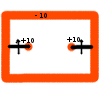
\includegraphics[width=0.2\textwidth]{img/rl_rewards}
   \end{figure}
   \item Value iteration: each vector has (extra) return value
   \item Updates:
   \begin{itemize}
    \item vector addition
    \item update last X vectors
    \item scale: value difference, last seen, normalize
   \end{itemize}
   \begin{figure}
    
\includegraphics[width=0.1\textwidth]{img/rl_add}
   \end{figure}
  \end{itemize}
\end{frame}

\section{Results}
\begin{frame}
 \frametitle{Results}
 Force fields
 \begin{figure}
  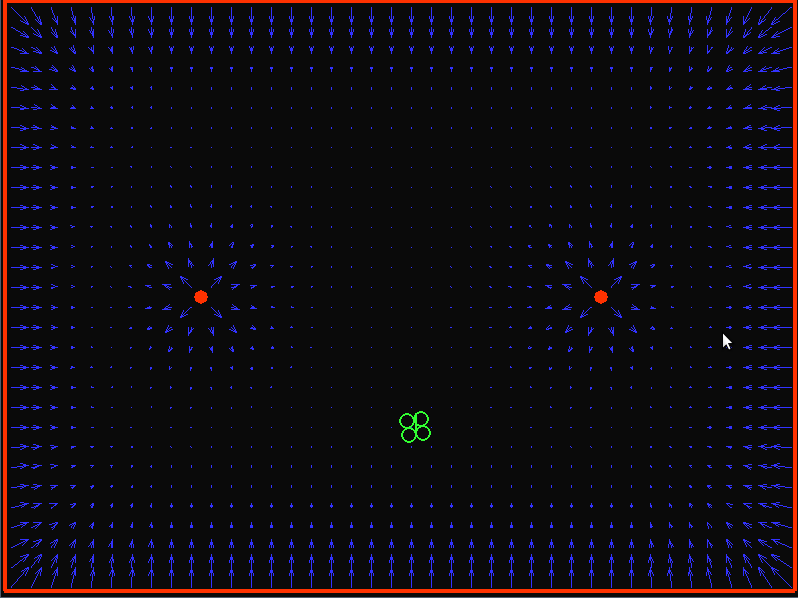
\includegraphics[width=0.7\textwidth]{img/force_fields}
 \end{figure}
\end{frame}

\begin{frame}
 \frametitle{Results}
 \begin{itemize}
  \item Level in unreal
  \item Writing code for Unreal
 \end{itemize}
 \begin{figure}
  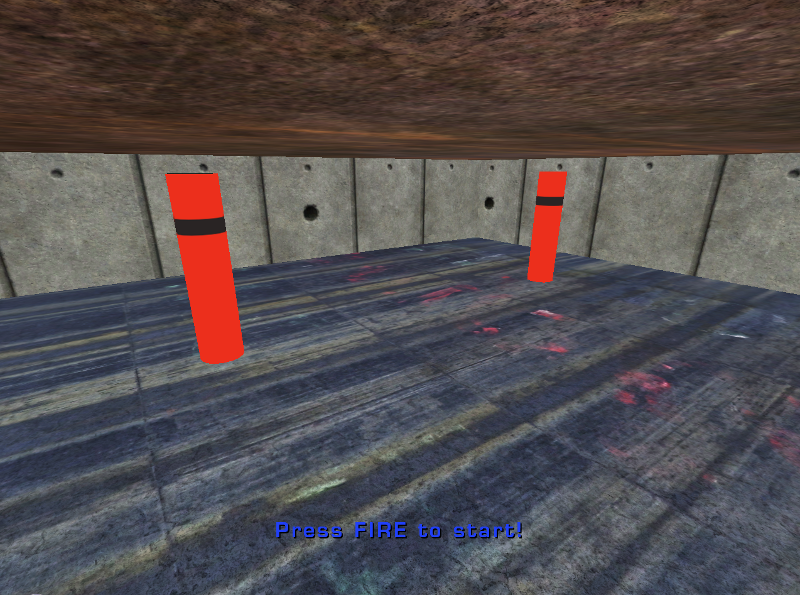
\includegraphics[width=0.7\textwidth]{img/unreal_pylonlevel}
 \end{figure}
\end{frame}

\section{Future Research}
\begin{frame}
 \frametitle{Future Research}
 \begin{itemize}
  \item lokalisatie (image matching, optical flow, RatSlam)
  \item IMAV2011 optimization (better level, etc)
 \end{itemize}
\end{frame}

\section{Summary}
\begin{frame}
\begin{block}{Questions?}
\end{block}
\end{frame}



\end{document}

